\documentclass{article}
\usepackage{graphicx} % Required for inserting images
\bibliographystyle{unsrt}

% table stuff
 \usepackage[normalem]{ulem}
 \useunder{\uline}{\ul}{}
 \usepackage[normalem]{ulem}
 \useunder{\uline}{\ul}{}
 \usepackage[normalem]{ulem}
 \useunder{\uline}{\ul}{}
 \usepackage[normalem]{ulem}
 \useunder{\uline}{\ul}{}
 \usepackage{float}

\title{NanoNeat}
\author{Przemysław Pilipczuk}
\date{December 2023}

\begin{document}

\maketitle

\tableofcontents
\section{Introduction}
\subsection{Abstract}
In this work I have implemented a fully functional  NeuroEvolution of Augumenting Topologies (NEAT) algorithm 
with a focus on simplicity and readibility. The implemenmtation aims to be a good resource for learning and teaching about NEAT.
The generic core algorithm is ~400 lines of Python code, and to adapt it to a specific problem requires about ~70 
more. I would argue that the terseness of source code makes it a good starting point for anyone interested in understanding NEAT, 
as it is easy to comprehend and easy to modify.
The implementation was tested on 4 problems: XOR, Cartpole, Acrobot and BipedalWalker. 

\subsection{Keywords}
Neuroevolution, NEAT, Evolutionary Algorithms, Machine Learning, Artificial Intelligence, Didactic Implementation
\section {The NEAT algorithm}
The NEAT algorithm, standing for NeuroEvolution of Augmenting Topologies, was first introduced in 2002 by Kenneth O. Stanley
and Risto Miikkulainen in their paper \cite{originalNeat}. This work not only proposed a novel approach to evolving neural
networks but also addressed some of the challenges faced by previous methods such as TWEANNs (Topology and Weight-Evolving
Artificial Neural Networks).
At the heart of NEAT is the principle of starting with the simplest possible network structure for each problem. Unlike previous
approaches that began with random and potentially complex structures, NEAT initializes with a basic network where the input
layer is fully connected to the output layer, devoid of any hidden nodes. This minimalistic starting point allows the algorithm
to incrementally and efficiently discover the necessary complexity, avoiding the pitfalls of starting with an overly complicated or suboptimal structure.
One of the main features of NEAT is the use of innovation numbers. This concept arose from the observation that systems
capable of evolving both topology and weights often represent similar solutions through vastly different structures and encodings.
This diversity, while beneficial for exploration, can hinder the effective combination of successful traits from different genomes.
To address this, NEAT assigns a unique global innovation number to each new connection in the population. This numbering system helps 
in identifying when two genomes independently evolve identical connections, thus facilitating more effective crossover by aligning similar structures.
Another critical aspect of NEAT is the concept of speciation. This mechanism ensures diversity within the population and prevents
premature convergence to local optima. In NEAT, the population is divided into species based on structural and weight differences
from a randomly chosen representative of each species. These species essentially represent subgroups of genomes exploring similar 
solutions, allowing NEAT to maintain a rich variety of strategies within the population. Speciation plays a crucial role in preserving
innovative structures that might otherwise be lost in a homogeneous population.
Furthermore, NEAT evaluates the fitness of each genome within the context of its species, a process termed "adjusted fitness."
This relative evaluation ensures that a single, highly fit species does not dominate the entire population, thereby maintaining
a healthy diversity of solutions and preventing stagnation in local minima. Adjusted fitness encourages the exploration
of various niches in the solution space, enabling the development of novel and potentially superior neural network architectures.
\section{Methodology}
    \subsection{Problems used to test the implementation}
        \subsubsection{XOR}
        Xor problem is a simple problem used mostly to test if the algorithm can start generating structure. 
        This is because XOR function is non linearly separable - it cannot be solved by the simple topology that neat starts with.
        To solve it, the algorithm needs to evolve a hidden layer. 
        This problem is thus used to test if the algorithm can generate minimal structure - the original paper \cite{originalNeat}
        states that the algoritm can solve the problem with 1 node in the hidden layer (However,
        it does require that the starting topology has an additional input node designated
        as bias, connected straight to the output). Both of these conditions are tested in this work.
        XOR problem is the ideal problem to test the various effects of the algorithm's configuration, as it is simple enough to be
        evaluated quickly even on home computers, and even running it for a thousand times is not a problem.
        \subsubsection{Cartpole}
        Cartpole is a problem taken from Farama Foundation's Gymnasium library \cite{gymnasium}. It is a classic control problem, 
        where an agent tries to balance a pole on a cart. The agent's observation space consists of cart's 
        position, velocity, angle of the pole and its angular velocity. The agent can move the cart left or right.
        This problem is a test of the implementation's ability to solve a basic real-world problem, but contrary 
        to the xor problem, its model is subjected to multiple sequential runs,
        with its fitness being judged based on its cumulative performance across these runs. This means, that
        recurrent connections can potentially be used.
        \subsubsection{Acrobot}
        Acrobot is a similar problem to the cartpole, with a slightly bigger state space. The problem consists
        of a two-link system, one of its ends fixed to a certain position. All of the joints are allowed to rotate,
        abd the agent is given control over an actuated joint between the two links. Its goal is to swing the
        end of the free link over given height (while starting from a hanging position). 
        THis problem also is evaluated as a single evaluation session, being subjected to multiple sequential runs,
        with its fitness being judged based on its cumulative performance across these runs.
        \subsubsection{BipedalWalker}
        BipedalWalker is the hardest problem used in this work. It is a problem taken from Farama Foundation's
        Gymnasium library \cite{gymnasium}. The agent tries to control a bipedal robot and make it walk to the end of the map, while
        making its movements energy-efficient. The observation space is significantly bigger than in previous problems,
        consisting of 24 values. The action space somewhat similar, but due to the problem specifics, requiring a 
        much more precise control. 
    \subsection{Implementation details}
        \subsubsection{Technology choices}
        The implementation is written in Python 3.11.5, and the dependencies needed for the core to work are:
        \begin{itemize}
            \item dill - used for serializing and deserializing particular genomes both for inspection and debugging purpouses. 
            \item networkx - used for creating the graph of the genome's tooplogy 
            \item pyvis - used for visualizing the graph of genome's topology
        \end{itemize}
        Additionaly, the problems sometimes require additional dependencies. Those being:
        \begin{itemize}
            \item gymnasium \cite{gymnasium} - used in cartpole, acrobot and bipedalwalker problems to simulate the environment
            \item torch \cite{Pytorch} - used in problems that require tweaking the activation function, as torch primitives enable easy control over the numerical precision. 
                It also enabled experiments with different approaches to evaluating a network - current implementation simply divides the genome into layers and 
                computes the output of each layer sequentially. This is not very performant, but it is easy to implement and understand. In the future,
                an alternative torch backend may be considered, where a genome compiles into a torch model, and then the evaluation is done by passing the input
                through it.
        \end{itemize}
        The choice of Python was made due to its simplicity and ability to convey the ideas of the algorithm in a concise way.
        Standard library of Python was used extensively to make sure the implementation is easy to follow.
        \subsubsection{Core algorithm}
        The core algorithm if NEAT is implemented in ~400 lines of Python in model.py
        The base for a single agent is a class called Genome. It contains a list of nodes and a list of connections for this particular 
        specimen, as well as a fitness value. Nodes and Connections have their own respectively named classes, both of which are accessing
        their Genomes' config object to get information about their ids and innovation numbers. Genome also controls the mutation process of itself,
        having separate methods for mutations of nodes, connections, and weights. Genome's config is a shared object between all genomes, and it is 
        given to it by a Population object during its initialization. Population is a class that controls the whole algorithm. It is responsible for
        maintaining a list of genomes, list of species, and maintaining a coherent state between all the mutations of genomes and changes in specie set.
        It is also responsible for the toplevel loop, that runs the algorithm for a given number of generations. The single iteration of that loop looks like this:
        \begin{enumerate}
            \item Divide the population into Species
            \item Calculate fitness of each individual genome
            \item Check for exit condition
            \item Calculate adjusted fitness of each individual genome
            \item Calculate offspring count for each specie
            \item Create new generation by crossover and mutation of selected genomes and species
            \item Repeat
        \end{enumerate}
        The Specie class is responsible for dealing with the speciation process and calculating relevant statistics for each (such as adjusted fitness or 
        generation without improvement count). 
        \subsubsection{Configuration}
        Population object is initialized with a Config object, which is a main way to configure algorithm. It is a simple object with a set of fields
        and a couple of methods. Most of the fields have default values, and are not required to be set manually by the user. The few fields that are
        mandatory are: 
        \begin{itemize}
            \item activation - the function used for activation
            \item input\_size - the number of input nodes
            \item output\_size - the number of output nodes
            \item experiment\_path - a path to where the experiment results will be saved
            \item fitness\_function - a function that takes a genome and returns its fitness
        \end{itemize}
        \begin{table}[H]
            \resizebox{\columnwidth}{!}{%
            \begin{tabular}{|l|l|l|}
            \hline
            \textbf{Variable name}               & \textbf{Default value} & \textbf{Description}                                                                                                                              \\ \hline
            c1                                   & 1                      & \begin{tabular}[c]{@{}l@{}}Modifier for excess genes count when calculating\\  distance between genomes\end{tabular}                              \\ \hline
            c2                                   & 1                      & \begin{tabular}[c]{@{}l@{}}Modifier for disjoint genes count when calculating\\  distance between genomes\end{tabular}                            \\ \hline
            c3                                   & 0.8                    & \begin{tabular}[c]{@{}l@{}}Modifier for weight differences when calculating\\  distance between genomes\end{tabular}                              \\ \hline
            meta                                 & \{\}                   & A dictionary to store problem-specific variables.                                                                                                      \\ \hline
            print\_generation                    &                        & \begin{tabular}[c]{@{}l@{}}A user-defined function for printing generation \\ during training\end{tabular}                                        \\ \hline
            every\_generation                    &                        & \begin{tabular}[c]{@{}l@{}}A function being executed after every generation.\\  Useful for saving information about learning\end{tabular}         \\ \hline
            after\_finished                      &                        & \begin{tabular}[c]{@{}l@{}}A function being executed after a problem\\  is finished\end{tabular}                                                  \\ \hline
            chance\_mutate\_weight               & 0.8                    & \begin{tabular}[c]{@{}l@{}}A chance for mutating weight during mutation\\  process\end{tabular}                                                   \\ \hline
            chance\_of\_20\_proc\_weight\_change & 0.9                    & Chance for a 20\% chance of weight value                                                                                                          \\ \hline
            chance\_of\_randomize\_weight        & 0.1                    & \begin{tabular}[c]{@{}l@{}}Chance for a completely new randomized value\\  for a given weight\end{tabular}                                        \\ \hline
            chance\_add\_connection              & 0.05                   & A chance to add a connection during mutation                                                                                                      \\ \hline
            chance\_add\_node                    & 0.05                   & A chance to add a node during mutation                                                                                                            \\ \hline
            tries\_to\_make\_connection          & 20                     & \begin{tabular}[c]{@{}l@{}}How many times system will try to find a valid\\  connection to make\end{tabular}                                      \\ \hline
            chance\_to\_reactivate\_connection   & 0.25                   & A chance to reactivate a disabled connection                                                                                                      \\ \hline
            allow\_recurremt                     & True                   & Allow forming recurrent connection                                                                                                                \\ \hline
            population\_size                     & 50                     & A size of population                                                                                                                              \\ \hline
            specie\_target                       & 4                      & A amount of species that system is trying to achieve                                                                                              \\ \hline
            max\_iterations                      & 600                    & \begin{tabular}[c]{@{}l@{}}A max amount of generation that system\\  is permitted to run for\end{tabular}                                         \\ \hline
            threshold\_step\_size                & 0.3                    & \begin{tabular}[c]{@{}l@{}}An amount that will be added or deleted to\\  threshold if specie size is higher or \\ lower than desired\end{tabular} \\ \hline
            problem\_fitness\_threshold          & 390                    & \begin{tabular}[c]{@{}l@{}}A threshold for fitness that will signify\\ that a genome has finished\\ successfully if exceeded\end{tabular}         \\ \hline
            top\_proc\_to\_reproduce             & 0.2                    & \begin{tabular}[c]{@{}l@{}}A percent of top genomes in every species' \\ that is enabled to reproduce\end{tabular}                                \\ \hline
            cross\_specie\_reproduction          & True                   & Can organisms pick partners out of their species                                                                                                  \\ \hline
            cross\_specie\_weight\_modifier      & 0.3                    & \begin{tabular}[c]{@{}l@{}}Modifier applied to chance of out-of-specie\\  reproduction\end{tabular}                                               \\ \hline
            enable\_elitism                      & True                   & \begin{tabular}[c]{@{}l@{}}Can best organisms in given generation be\\  passed to next generation\end{tabular}                                    \\ \hline
            elitism\_percentage                  & 0.05                   & \begin{tabular}[c]{@{}l@{}}How much of best organism from certain\\  generation can be passed to the next\end{tabular}                            \\ \hline
            dynamic\_threshold                   & True                   & \begin{tabular}[c]{@{}l@{}}A dynamic threshold tries to change\\  threshold to keep the specie size to\\  the given target\end{tabular}           \\ \hline
            initial\_threshold                   & 3                      & \begin{tabular}[c]{@{}l@{}}An initial threshold value for calculating\\  distance between two\\  genomes during speciation\end{tabular}           \\ \hline
            \end{tabular}%
            }
        \end{table}
        The fields presented here are all generic over the problem the algorithm is trying to solve. If a problem requires a specific configuration,
        (like a name of environment in gymnasium, or an offset for calculating fitness) it is stored in the meta field. This implementation was chosen
        to make sure users cannot accidentally overwrite an iternal field of the Config object, and also to provide a clear boundary between NEAT config 
        and problem-specific config, ensuring a more generic structure.
        \subsubsection{Problem-specific adjustments}
        \begin{itemize}
            \item XOR - This problem is given a custom activation function - a steepened sigmoid function.
            This is because in this problem we don't care about exact value of the output, but rather if it is closer to 0 or 1.
            The fitness function from origial NEAT paper \cite{originalNeat}, namely $$(4 - \sum_{n=1}^{4}c_n-o_n)^2$$
            where $c_n$ is the correct output and $o_n$ is the output of the network, for the problem's case number $n$.
            Recurrent connections are disabled.
            \item Cartpole - Here the configuration's meta field is used to store the name of the environment in gymnasium. That 
            variable is then used during Population initialization to create an environment. Fitness function then accesses that 
            environment to evaluate the genome.  
            \item Acrobot - Similarly to previous problem, configuration here utilizes meta field for Gymnasium's environment name. 
            Other than that, the configuration is standard with only mandatory fields being set.
            \item BipedalWalker - This problem required the most adjustments to the configuration. First of all, the fitness function 
            was tasked with offsetting the reward given by the environment, as its broad range of possible values was causing
            problems during adjusted fitness calculation, and therefore affecting mating pool selection. The fitness function was 
            programmed to cut minimum environment fitness value to a -100, and then offset that by 100 to make sure the fitness was always in range
            of 0-400. This fixed the problem of adjusted fitness calculation, but also forced us to increase the fitness threshold 
            for the problem by a 100. For clarity and coherent experience, custom printing function was used to print the 'environment' fitness
            for the problem, as it is more intuitive. During the testing of this setup, it was discovered that 
            the agent would often get stuck in an unrecoverable position and slow down the simulation by having to wait for the upper limit of time
            for the task to be reached. To fix this behavior, an additional variable was introduced to the model evaluation loop. It
            tracked the amount of timesteps since last improvement in the environment, and terminated the simulation if that number exceeded 
            a certain constant amount. This helped to increase the speed of learning, while not affecting the quality of the model in any way.
            Walker also needed its own activation function, as the baseline sigmoid function was not able to provide values in range [-1, 1].
            \end{itemize}
\section{Experimental results}
\begin{itemize}
    \item XOR
        \begin{table}[H]
            \resizebox{\columnwidth}{!}{%
            \begin{tabular}{|l|l|l|l|l|l|}
            \hline
                                                                                                 & Found solutions & \begin{tabular}[c]{@{}l@{}}Average generations \\ to completion\end{tabular} & \begin{tabular}[c]{@{}l@{}}Std. dev. generations \\ to completion\end{tabular} & \begin{tabular}[c]{@{}l@{}}average nodes\\ in final structure\end{tabular} & \begin{tabular}[c]{@{}l@{}}average connections\\ in final structure\end{tabular} \\ \hline
            Basic config                                                                         & 912 / 1000      & 124.94                                                                       & 63.40                                                                          & 9.48                                                                       & 20.59                                                                            \\ \hline
            Bias node added                                                                      & 834 / 1000      & 136.31                                                                       & 70.80                                                                          & 11.03                                                                      & 23.37                                                                            \\ \hline
            Dynamic threshold off                                                                & 634 / 1000      & 125.62                                                                       & 68.36                                                                          & 10.72                                                                      & 22.39                                                                            \\ \hline
            \begin{tabular}[c]{@{}l@{}}Dynamic threshold off\\  and bias node added\end{tabular} & 339 / 1000      & 132.03                                                                       & 72.10                                                                          & 12.55                                                                      & 25.57                                                                            \\ \hline
            \end{tabular}%
            }
            \end{table}
    \item Acrobot 
    Acrobot problem on default configuration solved the problem in all 1000 trials, with average
    generations being 4.45, standard deviation being 3.5. We also measured mean and standard deviation
    for the size of the structure that solved the problem. Average problem was solved in average of 8.95 nodes and 17.07
    connections, with respective standard deviations being 1.09 and 2.38.
    \item Cartpole
    Cartpole problem on default configuration solved the problem in all 1000 trials, with average
    generations being 2.77, standard deviation being 1.91. We also measured mean and standard deviation
    for the size of the structure that solved the problem. Average problem was solved in average of 5.06 nodes and 4.12 
    connections, with respective standard deviations being 0.31 and 0.66.

\end{itemize}
\section{Discussion}
From our results, there can be many conclusions. The problems do not constitute a linear progression of 
difficulty, and we can broadly say, that Acrobot and Cartpole problems were not complex enough for the network,
as a lot of the times they can be solved without evolving much of structure. They show, however that algorithm is capable
of exploring its current topology. 
\subsection{XOR trials}
    The results of XOR trials are suprising. They do show that the algorithm can solve the task, and that the default configuration is suitable for it.
    However, there are two things that are worth noting. First, the usage of a bias node seems to make the problem harder to solve, 
    which is the opposite of what we would expect. This could be due to the fact that having a bias node initially 
    makes the genome more susceptible to meaningless mutation of one more node and two more connections,
    instead of focusing on evolving the correct structure.
    \begin{figure}
        \centering
        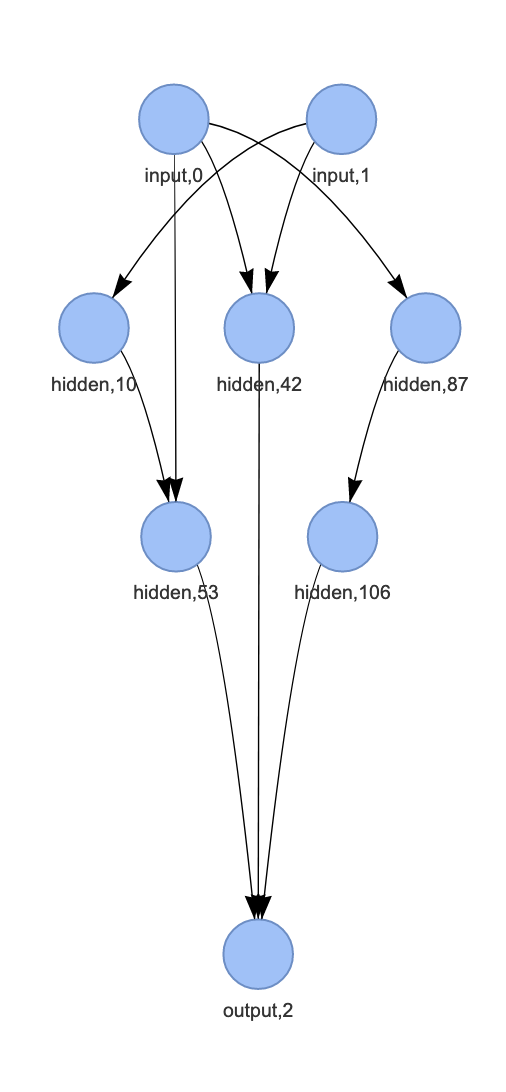
\includegraphics[width=0.8\textwidth]{xor_topology_example.png}
        \caption{An example topology of a genome that solves XOR problem without bias node }
        \label{fig:xor_bias}
    \end{figure}
    Second, the lack of dynamic threshold for specie distance calculation seems to make the problem harder to solve.
    This is less suprising, as the dynamic threshold is a mechanism that is supposed to help the algorithm in situations
    where the problem is hard to solve. What is suprising about this is that the difference in performance is so big for
    such a simple problem. This solution is also not very robust compared to the original one, achieving only 91.2\% success rate
    compared with 100\% of the original, and taking far more generations to find the solution.
\subsection{Cartpole}
    The results of cartpole trials are not very useful. The problem is solved in all 1000 trials, but the results suggest, that 
    this problem is too easy for the algorithm to be a good test of its capabilities. The average number of generations is 2.77, 
    meaning that the algorithm is able to solve the problem in less than 3 generations on average. To solve cartpole problem, the
    algorithm doesn't need to evolve any structure, as the starting topology is enough to solve the problem. The problem is therefore
    not inspected further.
\subsection{Acrobot}
    Solution to the acrobot problem is showing more promise than the cartpole, but ultimately also fails to provide a 
    good challenge to the algorithm. The problem is solved in all 1000 trials, and even though the average number of generations is up, it 
    is still only 4.45. The average number of nodes and connections in the solution is also very low, with 8.95 and 17.07 respectively. 
    Given that the minimal starting genome for this problem has 8 nodes and 15 connections, it is safe to say this problem can be 
    categorized as trivial.
\subsection{Walker}
    The case of bipedalwalker is a curious one. The model can reliably learn to walk to the end of the map (corresponding
    to this is fitness of about ~150-200). It cannot however finish the course with a cumulative fitness required by the
    environment. How is that possible? The environment in bipedalwalker has total fitness requirement of 300, divided
    into small chunks given to an agent by moving forward. However, environment also keeps track of the movement made
    by the agent, and reduces reward based on the 'energy-efficiency' of its movements. In this situation agent 
    gets terminated by the environment (has walked to the end of the map), but doesn't have enough fitness to be 
    qualified as a win. 
    This is problematic, as the fitness function used by the algorithm (and the gymnasium environment
    itself) is not suited well for teaching agents to walk efficiently. There is enough noise inbetween
    randomly generated maps, that the difference in fitness from a good run and a bad run is more reliant
    on the map itself than the agent's efficiency in performance.
     That is because once the agent learns to walk, the reward it gets from simply moving forward is higher than any influence
     of the energy-efficiency correction. This means that the agent is not incentivized to walk efficiently, and
     once it gets to the end of the map consistently, there is no clear way for it to improve its fitness (the 
     act of walking efficiently seems to need far more structure, which is hard to evolve when there is small 
     reward to be gained at this point.
      )
    are very long, with the fitness being reduced by the environment constituting a very small part of the total fitness missing.
\section{Future work}
    Proposed future work is divided into two categories: 
        \subsection{Improvements to the visualization} 
        To make the didactic part of the implementation more useful, it would be good to add a visualization of the
        learning process. Current version permits user to dump data from the learning process, which is used to
        generate graphs representing state of the select genomes in the network. This is a good start, but is not
        a very user-friendly way of interacting with the system. It would be better to have a live visualization.
        Currently in the codebase, there is also no code for plotting the specie perormance over time, which would
        help in understanding the speciation process.
        \subsection{Improvements to the performance}
        The current implmenentation focused on simplicity, and therefore is not very performant. And while performance
        is not a stated priority, it there are some ways to improve it without sacrificing much of the simplicity.
        The evaluation of the genomes is currently done in a single thread, which is a bottleneck for the whole process.
        It would be good to implement a multithreaded evaluation, which would speed up the process significantly.
\section{Bibliography}
\bibliography{references}
\end{document}